\section{Pruebas al modelo de reconocimiento facial sobre conjuntos de datos personales}

Una vez que se seleccionó la configuración ideal, después de validarlo con un subconjunto del dataset LFW con 1000 entidades, procedimos a evaluarlo con algunas imágenes de rostros de nuestra comunidad estudiantil.\\


La configuración del sistema de reconocimiento facial y la metodología de evaluación se establecieron con los siguientes parámetros clave:


\subsection{Directorio de Imágenes}
Todas las imágenes utilizadas para el registro y la evaluación del sistema se organizan en un directorio base:
\begin{itemize}
	\item \texttt{BASE\_IMAGES\_DIR = 'imagenes\_alumnos'}
\end{itemize}
Dentro de este directorio, se espera una subcarpeta por cada individuo (ej., \texttt{2022630082}), conteniendo dos tipos de imágenes:
\begin{itemize}
	\item \texttt{*\_new.png}: Imagen utilizada para el registro del individuo (extracción del embedding de referencia).
	\item \texttt{*\_old.png}: Imagen utilizada para la evaluación (simula una nueva captura a ser identificada).
\end{itemize}

\subsection{Modelo de Reconocimiento Facial}
Para la extracción de los \textbf{embeddings faciales}, se seleccionó uno de los modelos pre-entrenados más robustos disponibles en \texttt{DeepFace}:
\begin{itemize}
	\item \textbf{Nombre del Modelo (MODEL\_NAME):} \texttt{Facenet}
\end{itemize}
\texttt{Facenet} es conocido por su alta precisión en la tarea de verificación facial al generar representaciones vectoriales densas (embeddings) de los rostros.

\subsection{Backend del Detector Facial}
Para la detección y alineación de los rostros dentro de las imágenes antes de la extracción del embedding, se utilizó el siguiente detector:
\begin{itemize}
	\item \textbf{Detector Backend (DETECTOR\_BACKEND):} \texttt{fastmtcnn}
\end{itemize}
\texttt{fastmtcnn} es una opción eficiente que busca un equilibrio entre velocidad y precisión en la detección de rostros.

\subsection{Métrica de Distancia y Umbral}
La comparación entre los embeddings se realiza utilizando una métrica de distancia específica, y se aplica un umbral para determinar si dos rostros pertenecen a la misma persona:
\begin{itemize}
	\item \textbf{Métrica de Distancia (DISTANCE\_METRIC):} \texttt{cosine}
\end{itemize}
La distancia coseno ($D_c$) se calcula como $1 - \text{similitud\_coseno}$, donde la similitud coseno es el coseno del ángulo entre dos vectores. Valores cercanos a 0 indican alta similitud (distancia pequeña).
\begin{itemize}
	\item \textbf{Umbral de Distancia (DISTANCE\_THRESHOLD):} \texttt{0.4}
\end{itemize}
Un valor de distancia coseno \textbf{menor o igual} a este umbral indica que los dos embeddings corresponden al mismo individuo. Este umbral es crucial para la decisión de identificación.

---

\section{Propósito del Experimento}

El propósito fundamental de este experimento es:

\begin{enumerate}
	\item \textbf{Evaluar la Precisión de Identificación:} Determinar cuán exitosamente el sistema puede identificar a los alumnos registrados utilizando imágenes diferentes a las de registro (\texttt{*\_old.png}). Esto implica medir la capacidad del sistema para clasificar correctamente cada imagen de prueba con su identidad verdadera.
	
	\item \textbf{Medir el Rendimiento de Clasificación:} Utilizar métricas estándar como \textbf{precisión}, \textbf{exhaustividad (recall)} y \textbf{puntuación F1} para cada clase (cada alumno registrado), así como la \textbf{exactitud (accuracy)} general del sistema.
	
	\item \textbf{Comprender el Comportamiento ante "Desconocidos":} Aunque en este conjunto de datos inicial no se incluyen explícitamente imágenes de "desconocidos" para la evaluación, el sistema está diseñado para clasificarlos como tal si no encuentran un match por debajo del umbral. La matriz de confusión y el reporte de clasificación permitirán observar cómo se manejarían estos casos, incluso si el soporte actual para esta clase es nulo. Este es un punto clave para futuras expansiones del conjunto de datos de prueba.
	
	\item \textbf{Validar la Configuración de Umbral:} Observar el impacto del \texttt{DISTANCE\_THRESHOLD} en las decisiones de identificación. Un umbral bien ajustado es vital para minimizar tanto los \textbf{falsos positivos} (identificar erróneamente a alguien) como los \textbf{falsos negativos} (no reconocer a alguien registrado).
	
	\item \textbf{Generar una Matriz de Confusión:} Visualizar gráficamente el rendimiento del clasificador para cada clase, mostrando las identificaciones correctas e incorrectas, lo cual es fundamental para el análisis de errores.
\end{enumerate}


\begin{figure}[htbp]
	\centering
	\begin{subfigure}[b]{0.48\textwidth} % La [b] es para alinear en la parte inferior, 0.48\textwidth para dejar un pequeño espacio entre ellas
		\centering
		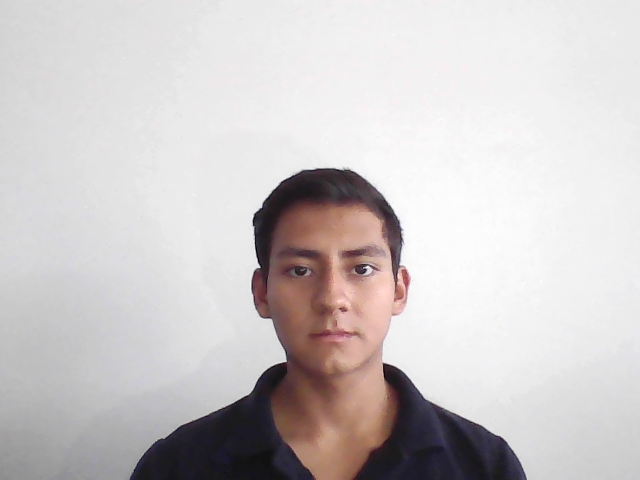
\includegraphics[width=\textwidth]{images/2022630467_new.png}
		\caption{Imagen registrada en el sistema (ej., Imagen de Registro)}
		\label{fig:primera_imagen}
	\end{subfigure}
	\hfill % Para distribuir el espacio horizontalmente
	\begin{subfigure}[b]{0.3\textwidth}
		\centering
		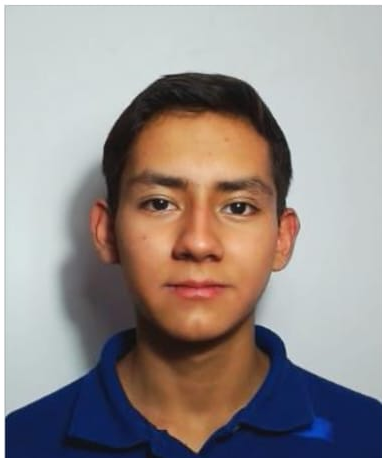
\includegraphics[width=\textwidth]{images/2022630467_old_crop.png} 
		\caption{Imagen de prueba (ej., Imagen de Prueba)}
		\label{fig:segunda_imagen}
	\end{subfigure}
	\caption{Conjunto de imágenes mostrando un ejemplo de imagen de registro y su correspondiente imagen de prueba.}
	\label{fig:conjunto_imagenes}
\end{figure}
